\documentclass[a4paper,12pt]{report}
\usepackage{graphicx}
\usepackage[utf8]{inputenc}
\usepackage{url}
\usepackage[italian]{babel}
\usepackage[italian]{cleveref}

\title{Elaborato per il corso Basi di Dati\\ \small Progetto di una base di dati per la gestione di un sito di e-Commerce}

\author{
    Studente: Emma Leonardi\\
    Email: \url{emma.leonardi2@studio.unibo.it}\\
    Matricola: 0000971438\\
    A.A. 2021/2022
    }
\date{}
\begin{document}

\maketitle
\tableofcontents

\chapter{Analisi}
\section{Analisi dei requisiti}
Si ha intenzione di creare un database per gestire un sito di e-Commerce.
Il database dovrà memorizzare informazioni sui prodotti in vendita, gestire l'interazione con il cliente che compra i prodotti. 
Inoltre dovrà gestire anche i corrieri che effettuano le consegne delle spese e sapere in quale fabbrica viene prodotto quale prodotto.
\section{Intervista}
Si vuole tenere traccia degli acquisti dei clienti. I dati dei clienti memorizzati sono nome, cognome, codice fiscale, data di nascita, 
email e numero di telefono, coordinate bancarie e indirizzo di residenza.
Il cliente acquista una spesa con un costo che è la somma dei costi dei prodotti presenti nella spesa. 
I prodotti possono cambiare prezzo nel tempo e bisogna tenere memorizzato lo storico. 
Dei prodotti si salva il materiale, la descrizione, la taglia se abbigliamento o la scadenza se prodotto alimentare. 
I prodotti vengono creati in fabbriche, gestite da più produttori in periodi diversi. Una fabbrica viene gestita da un solo produttore alla volta e può produrre diversi prodotti. 
Del produttore si salva la partita IVA e della fabbrica l'indirizzo. Un prodotto viene fabbricato in una sola fabbrica.
La spesa viene consegnata da un corriere e si salva la data. Un corriere guida un mezzo, di cui si memorizzano il tipo di veicolo, la marca, il paese di immatricolazione e la targa.
Del corriere vengono memorizzate la nazionalità della patente, il codice e i turni di guida. La consegna può essere standard o premium, cambia il prezzo della consegna.
La consegna ha collegato un indirizzo, che può essere diverso dall'indirizzo di residenza del cliente. Più corrieri non possono guidare lo stesso mezzo in contemporanea, la consegna è effettuata da un unico corriere 
e si riferisce ad una sola spesa. Una spesa è riferita a un solo cliente, ma un cliente può effettuare più spese. 
Si memorizzano nome, cognome, codice fiscale e data di nascita per i clienti, produttori e corrieri.


\section{Rilevamento delle ambiguità e correzioni proposte}
Correzoni
\section{Definizione delle specifiche in linguaggio naturale ed estrazione dei concetti principali}
Estrazione concetti\\
Tabella termini-> concetto, correzione

\chapter{Progettazione Concettuale}
\section{Schema scheletro per Clienti}
Dopo aver esaminato il dominio del problema per la parte dei clienti, viene proposto il seguente schema scheletro.
\begin{figure}[h]
	\centering{}
	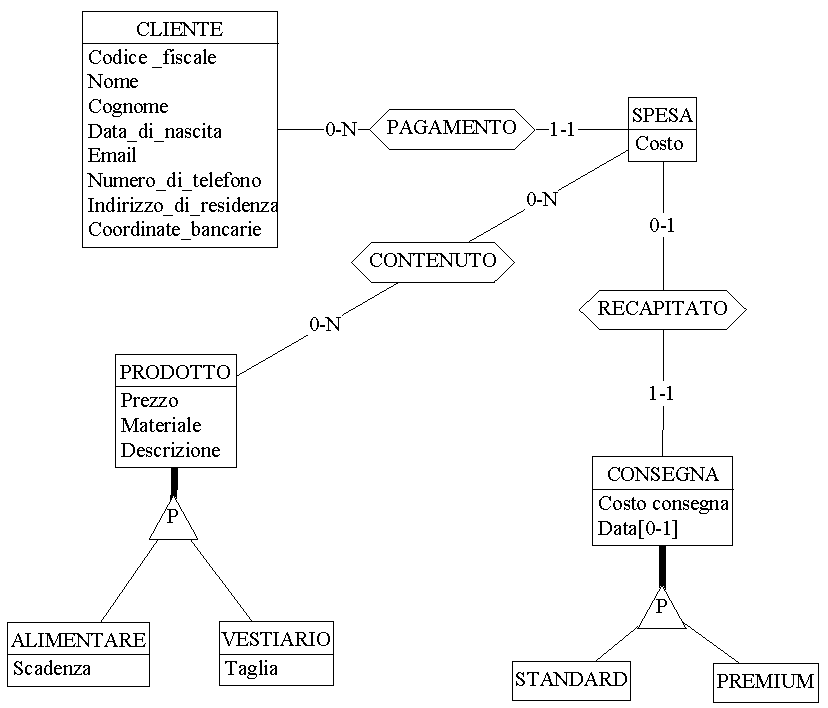
\includegraphics[width=\textwidth]{img/SchemaConcettuale-Clienti1.pdf}
	\caption{Schema scheletro per i Clienti}
\end{figure}
\section{Raffinamenti proposti per clienti}
L'entità Cliente è una estensione di un'entità generica Persona, che si decide di aggiungere allo schema. 
L'entità Prodotto non permette di mantenere uno storico dei diversi prezzi e delle diverse "versioni" dello stesso prodotto, come la taglia o la scadenza. 
Per questo si decide di creare un'entità Prodotto in Vendita che è il prodotto venduto al cliente, collegato al Prodotto e si aggiungono al Prodotto in Vendita il prezzo e il periodo di validità del prezzo. 
Come identificatori per l'entità cliente si usa un codice univoco (per evitare l'omocodia del codice fiscale), per Spesa e Prodotto si usa un codice univoco e per Consegna si usa come identificatore 
l'identificatore importato di Spesa con la data.
\section{Schema concettuale parziale per clienti}
\begin{figure}[h]
	\centering{}
	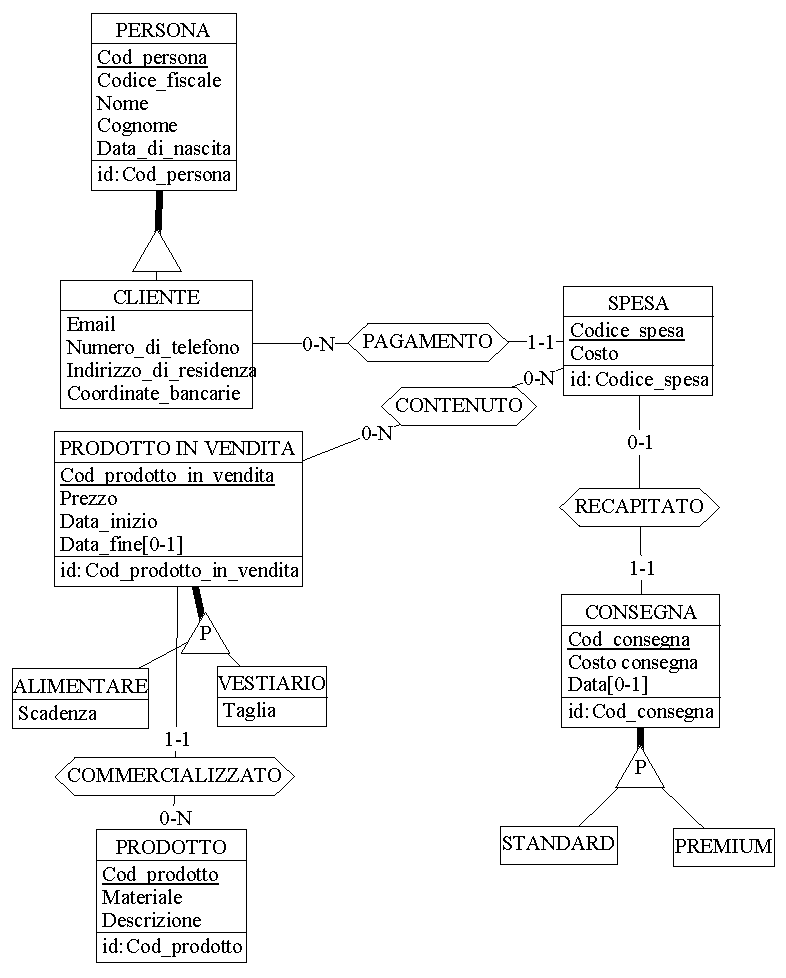
\includegraphics[width=\textwidth]{img/SchemaConcettuale-Clienti2.pdf}
	\caption{Schema scheletro per i Clienti, dopo le modifiche apportate}
\end{figure}
\section{Schema scheletro per Corrieri}
Dopo aver esaminato il dominio del problema per la parte dei corrieri, viene proposto il seguente schema scheletro.
\begin{figure}[h]
	\centering{}
	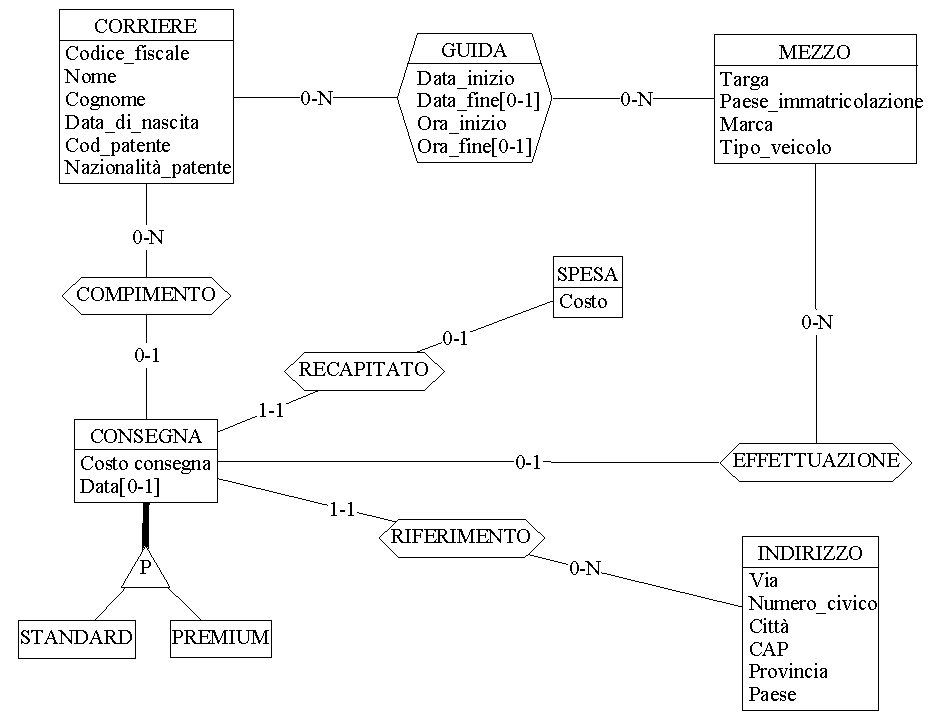
\includegraphics[width=\textwidth]{img/SchemaConcettuale-Corrieri1.pdf}
	\caption{Schema scheletro per i Corrieri}
\end{figure}
\section{Raffinamenti proposti per corrieri}
L'entità Corriere è una estensione di un'entità generica Persona, che si decide di aggiungere allo schema. 
La relazione Guida non è corretta rappresentata come relazione perchè questo impedisce ad un corriere di guidare lo stesso mezzo più volte. Guida diventa una entità quindi, in relazione 1-1 con Corriere e Mezzo, mentre le cardinalità dai lati delle entità rimangono 0-N. 
Come identificatori per Corriere si può usare il codice di persona oppure il codice della patente. 
Per Mezzo come identificatore uso la Targa, per Guida un codice univoco, per Consegna si usa come identificatore l'identificatore importato di Spesa con la data. 
L'identificatore di Spesa è un codice, anche per indirizzo.
\section{Schema concettuale parziale per corrieri}
\begin{figure}[h]
	\centering{}
	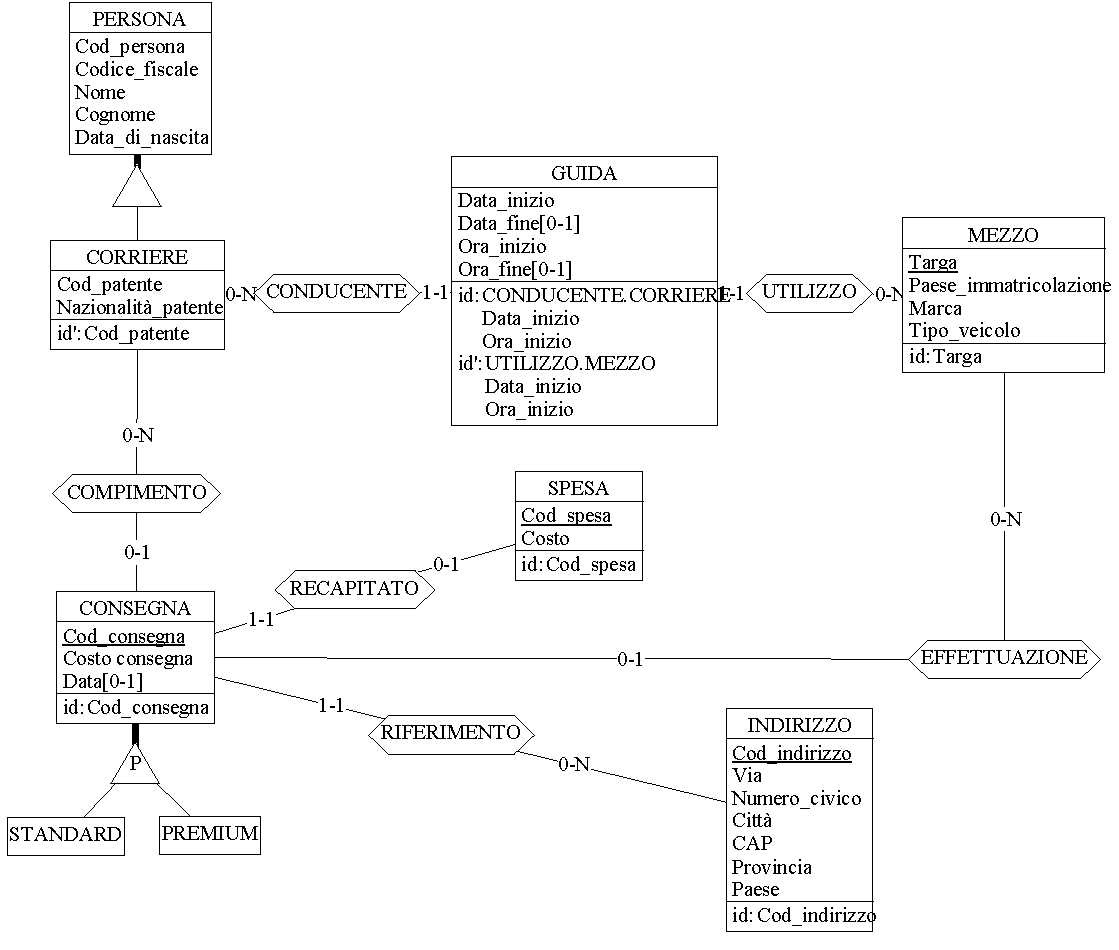
\includegraphics[width=\textwidth]{img/SchemaConcettuale-Corrieri2.pdf}
	\caption{Schema scheletro per i Corrieri, dopo le modifiche apportate}
\end{figure}


\section{Schema concettuale finale}
ER finale

\chapter{Progettazione Logica}
\section{Stima del volume dei dati}
Tabella volume
\section{Descrizione delle operazioni principali e stima della loro frequenza}
Tabella op frequenza
\section{Schemi di navigazione e tabelle degli accessi}
Conti pesantezza operazioni, con tabelle
\section{Raffinamento dello schema}
eliminazione di identificatori esterni, attributi composti e gerarchie, scelta delle chiavi
subsection per ognuno di questi lavori
\section{Analisi delle ridondanze}
Ridondanze, conti
\section{Traduzione di entità e associazioni in relazioni}
Traduzione ER
\section{Schema relazionale finale}
Schema finale
\section{Traduzione delle operazioni in query SQL}
delle operazioni

\chapter{Progettazione dell'applicazione}
\section{Descrizione dell'architettura dell'applicazione}
Java, operazioni banali (inserimento, ecc)
realizzata con obbligo di inserire alcuni screenshot dell'interfaccia utente
diverse schermate (utente, corriere, ecc)
tabella operazione originale -> metodo/classe
\end{document}